\chapter{THE REVERSE MAPPING PROBLEM}
\thispagestyle{plain}

\label{ReverseMapping}

The reverse-mapping problem is the problem of defining a function $f^{-1}$ that maps a system-level configuration $\mathbf y$ onto a solution space $\hat{\mathbf S}$ that represents all possible configurations that would have the system exhibit $\mathbf y$:
   \[ f^{-1}(\mathbf y) \rightarrow \hat{\mathbf S}. \]
Every configuration $\hat {\mathbf x} \in \hat {\mathbf S}$ should satisfy the constraint $f(\hat{\mathbf x}) \approx \mathbf y$, where $f$ is the forward mapping.
That is, $\hat{\mathbf S}$ contains all the points that would predict $\mathbf y$ in the forward mapping.

In this chapter, I give details of how \fw approaches the solution to this problem, in general, then delves deeper into actual implementations of the solution.
Then, I discuss evaluation criteria for implementations of reverse-mapping problem solutions.

\section{The \fw Approach}

The general approach taken by \fw for solving the reverse-mapping problem is similar to the \fw forward-mapping solution approach.
First, the different system-level properties are split into sub-problems.
Next, solution spaces for each sub-problem are constructed with a forward-mapping inversion technique.
Finally, each solution subspace is recombined to produce the space of configurations that will produce the provided system-level property.

Much like the forward-mapping solution, $\mathbf y$ is split into subspaces to simplify the problem:
\[ \mathbf y = \{y_0, y_1, \ldots, y_{|\mathbf y|}\}. \]
The solution space is split up in a similar manner:
\[ \hat{\mathbf S} = \{\hat S_0, \hat S_1, \ldots, \hat S_{|\mathbf S|}\}. \]
By performing this split, each forward mapping can be inverted independently:
\[ f^{-1}_i(y_i) \rightarrow \hat S_i. \]

Recombining the individual $\hat S_i$ into $\hat{\mathbf S}$ is not as simple as recombining individual $\hat y_i$ into $\hat{\mathbf y}$ in the forward-mapping solution.
Since each solution space represents which configurations satisfy a particular system-level requirement, the solution space $\hat{\mathbf S}$ is the intersection of all these spaces:
\[ \hat{\mathbf S} = \hat S_0 \cap \hat S_1 \cap \ldots \cap \hat S_{|\mathbf S|}.\]
All points at the intersection of these spaces should satisfy all system-level properties at once.

The nature of the solution spaces vary from approach to approach.
In the approaches used by \fw, they are represented as a collection of discrete subspaces, discrete exemplar points, sets of functions, or linear combinations.

\section{Approaches}

I have devised and evaluated a number of different approaches for solving the reverse-mapping problem in this dissertation research.
This section enumerates these approaches.
Although each the approaches are quite different, they all \textit{invert} a solution to the forward-mapping problem.
That is, they use the forward mapping to develop the reverse mapping, instead of learning the reverse mapping directly.
This has the benefit that the reverse-mapping solutions are agnostic to the regression method used to learn the forward mapping.

Each approach is follows a different technical process, but all query the forward mapping for points instead of using the original data set.
Most approaches conform to the assumption stated in Chapter \ref{ForwardMapping}: The Forward-Mapping Problem that all the system-level properties can be analyzed independently.
Every approach has a different method for intersecting the different solution spaces to find a solution space that satisfies all system-level properties at once.

Each approach has different computational and space complexity.
The expectations for each method and the situations in which they are optimal vary from domain to domain and from query to query.

The first two approaches discussed in this section, \textit{Thresholding} and \textit{Regression} / \textit{Interpolation} / \textit{Intersection}, conform to the theoretical framework outlined above.
Two other approaches are labeled as alternatives, as they do not follow the framework exactly, but perform a similar task.
In the final subsection, I discuss the special case in which the system-level property is a binary value (i.e., the forward mapping is classification).
Throughout this section, I use the NetLogo Fires ABM\footnote{More on the Fires model is discussed in Section \ref{sec:Fires}} as an example.
The Fires domain is simple, but has solution spaces that are easy to visualize.
Other domains, such as Wolf Sheep Predation, have too many dimensions possibly graph.
The arguments made with the aid of the Fires domain scale to larger dimensions.


\begin{figure}[ht]
\centering
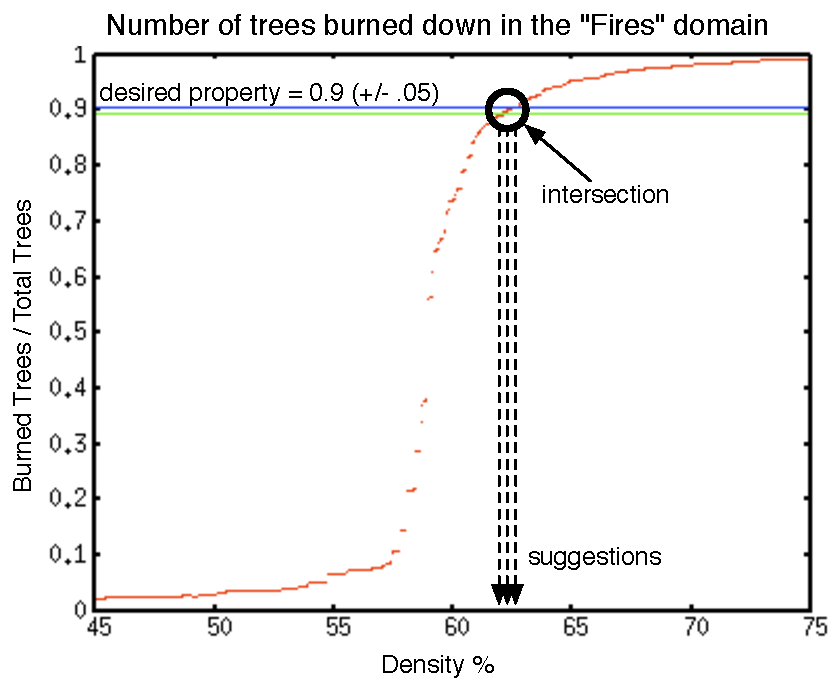
\includegraphics[scale=.66666667]{images/firesthreshold.pdf}
\caption{An illustration of the \textit{thresholding} approach to the reverse-mapping problem.}
\label{fig:firethresh}
\end{figure}

\subsection{Thresholding}

The simplest of the approaches discussed in this dissertation is dubbed the \textit{thresholding} approach.
In this approach, all points within some margin $\varepsilon$ from the system-level property $y$ are returned.
For example, all sampled points near .9 would be returned if we wanted a configuration that would yield about 90\% of the trees burned down in the Fires ABM.
Figure \ref{fig:firethresh} is an illustration of applying the thresholding approach to a data set collected for the Fires domain.
The points within this threshold are an approximation of the \textit{intersection} between the $y=.9$ plane (the horizontal lines) and the behavior space (the dots).
Configuration points that are part of this intersection are expected to produce values close to $y=.9$.
In a 600 point data set and $\varepsilon=.005$, nine points are returned that suggest configurations from 62.1 to 62.5.

This approach typically requires a large data set.
With smaller data sets, sometimes a threshold may not contain any points where there is a lot of change.
For example, no points exist between .4 and 5.5 in the 600 point data set shown in Figure \ref{fig:firethresh}.
Also, in a domain with some variance, some outliers from distant parts of the space may be included in within the threshold.
To remedy this situation, the data set can be augmented (or replaced) with a multitude of inferred points by using the forward mapping.
The data set shown in \ref{fig:firethresh} consists of interpolated points, instead of raw points (see \ref{fig:rii0} for a comparison).
The size of this data set can be made arbitrarily large given enough computation time.
Now, the threshold approach can be used and a large number of points will be returned.

There is another benefit to using inferred points over the raw data points.
The inferred points are ``smoothed" because the magnitude of the errors from neighboring points effectively cancel each other out.
These points will be even more accurate than the raw points, assuming that the forward mapping does not exhibit unseen bias.
This is because inferred points may be closer to the mean than their raw counterparts.

This approach requires O($N$) time (where $N$ is the number of points in the data set) because each point is checked to see whether it lies within the threshold.
This process can be sped up dramatically by segregating the configuration space into discrete bins.
For each bin, the minimum and maximum values for the system-level property are noted.
Now, instead of checking each point, each bin is checked to see if it could possibly contain points of the given system-level property value (i.e., the desired value is between the minimum and maximum values of the bin).
Once the candidate bins have been selected, the points in the individual bins are inspected more closely.
The same points are returned that would have been returned with the naive implementation, but without having to scan many of the points.
The pre-processing step of segregating points into bins is done offline once, and thus its computational requirement is amortized over all queries.

In comparison to the next approach discussed in this chapter, thresholding is the simplest to implement.
However, the mapping is a set of discrete points, which has limited usefulness.
Additional techniques must be applied to the solution set in order to gain any sort of high-level view.

\subsection{Regression/Interpolation/Intersection}

Perhaps the most advanced technique \fw uses to solve the reverse mapping is \textit{Regression/Interpolation/Intersection} (RII).
This approach has three phases.
First, regression is used to infer the system-level property values for several evenly spaced ``knots" in the configuration space.
Next, multi-linear interpolation is set up in each hypercube formed by connecting the knots.
Finally, each piecewise region is ``inverted" to build a gradient across the behavior space that represents a $y$ value of interest.

\begin{figure}[ht]
\centering
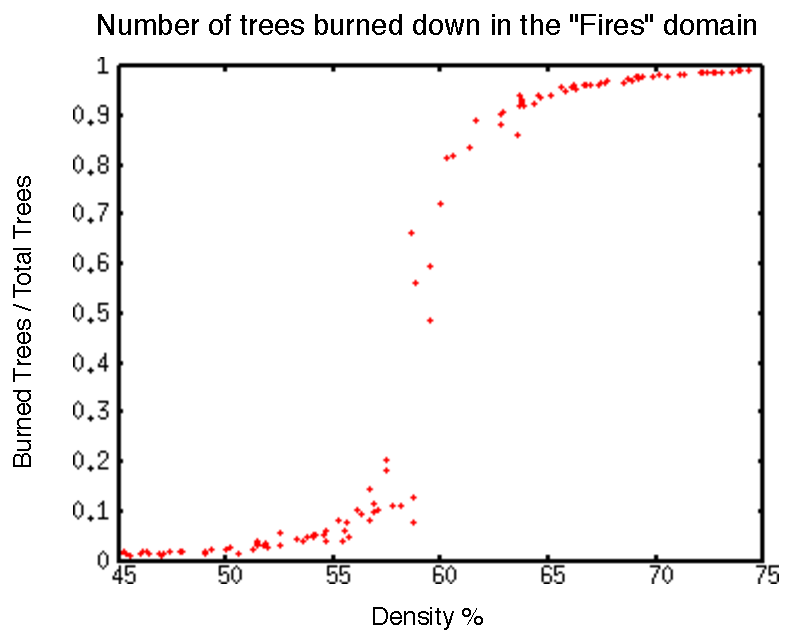
\includegraphics[scale=.66666667]{images/rii0.pdf}
\caption{The raw data set, containing 120 points, from the Fires domain.}
\label{fig:rii0}
\end{figure}

\begin{figure}[ht]
\centering
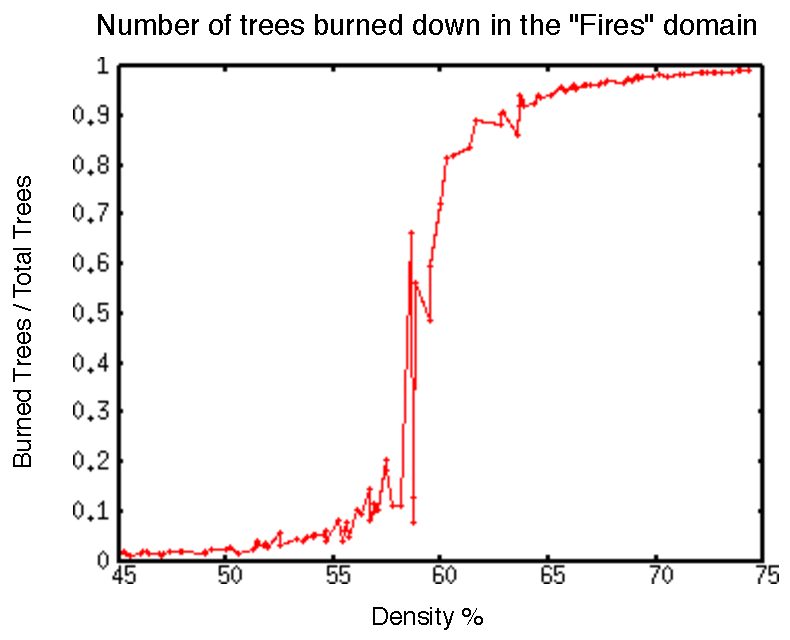
\includegraphics[scale=.66666667]{images/rii1.pdf}
\caption{Linear interpolation performed on the raw data set (see Figure \ref{fig:rii0}) from the Fires domain.}
\label{fig:rii1}
\end{figure}

The reason for using regression as the first step is the same as for using inferred points instead of the raw data set in the threshold approach.
The raw data in many ABMs will exhibit some variance.
For example, raw data from the Fires ABM is shown in Figure \ref{fig:rii0}
If this data were to be used when interpolating, the curve for the behavior space would be very erratic.
This is a problem for RII because erratic curves will result in a number of inaccurate intersections.
A linear interpolation performed on the raw Fires data to generate a behavior space curve is shown in Figure \ref{fig:rii1}.

\begin{figure}[ht]
\centering
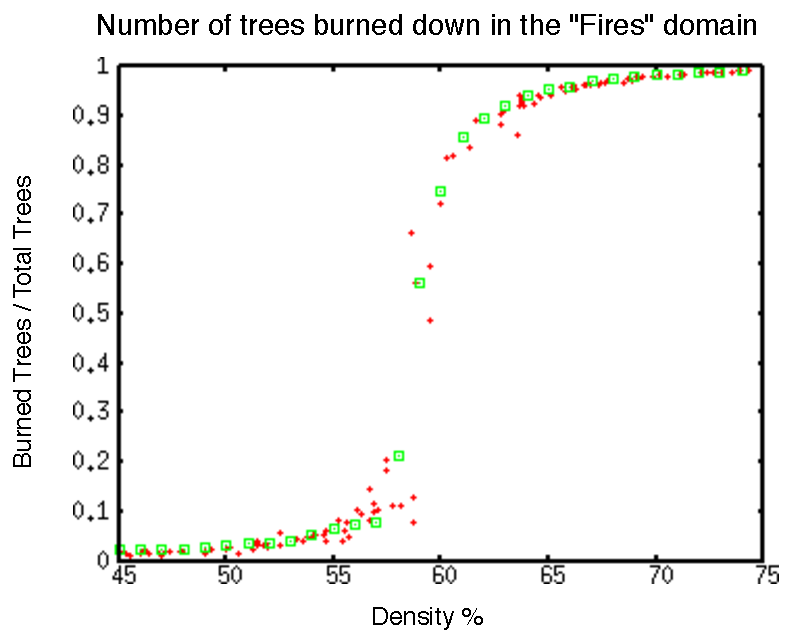
\includegraphics[scale=.66666667]{images/rii2.pdf}
\caption{Knots (squares) for the Fires domain that have been inferred by the forward mapping.}
\label{fig:rii2}
\end{figure}


The curve is naturally much smoother when regression is used.
The first step is to use the forward mapping (i.e., regression) to infer evenly spaced knots in the space.
These knots canvas the space and provide reference points for the interpolation.
As the dimensionality of the configuration space increases, the number of knots increases:
Hypercubes will have $2^d$ corners and thus will require $2^d$ knots, each.
For example, in the Fires domain, the configuration space is one dimensional.
Therefore, the hypercubes formed by the knots are line segments.
Knots spaced every 1\% that have been inferred from the raw Fires data is shown in Figure \ref{fig:rii2}.

Next, the minimum and maximum values of the system-level property is recorded for each separate hypercube in the configuration space.
This is done by iterating through every corner of the hypercube and taking the maximum and minimum value for their inferred system-level property value.
This enables the intersection step to decide which hypercubes intersect with the desired system-level property value.
A plane must intersect with the cube if the system-level property value is between the maximum and minimum, assuming continuity within cubes (intermediate value theorem).
For example, the only section of the Fires domain that need to be checked for the \textit{Burned Trees / Total Trees} value of 0.15 is between 57\% and 58\%.
This region is the only one in the space that could possibly intersect with the value .15, because it has a minimum value of .08 and a maximum value of .21.
Many more intersecting hypercubes are expected in ABMs higher dimensional configuration spaces.
The entire process of inferring the knots and noting the minimum and maximum values is done offline.
Therefore, the computational time required by this step is negligible when amortized over a number of reverse-mapping queries.

\begin{figure}[ht]
\centering
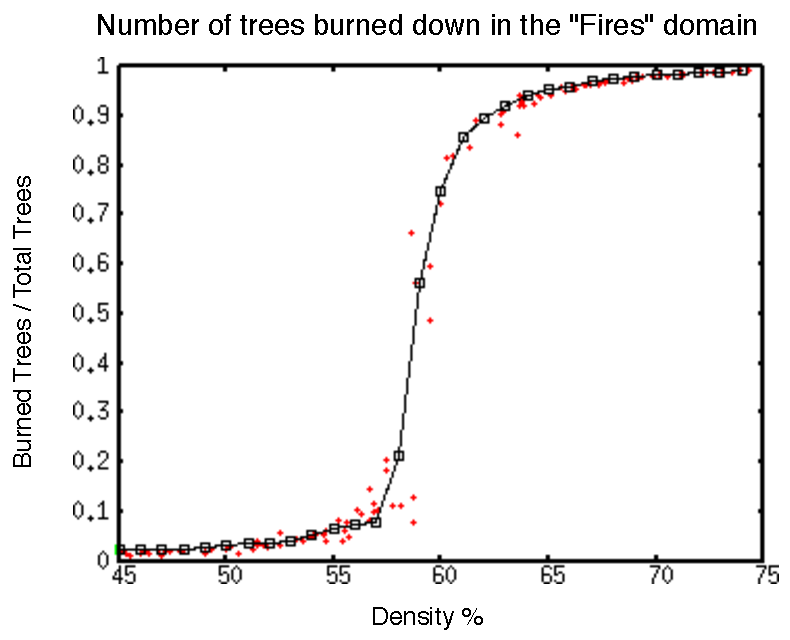
\includegraphics[scale=.66666667]{images/rii3.pdf}
\caption{Gradients between the knots for the Fires domain}.
\label{fig:rii3}
\end{figure}

\begin{figure}[ht]
\centering
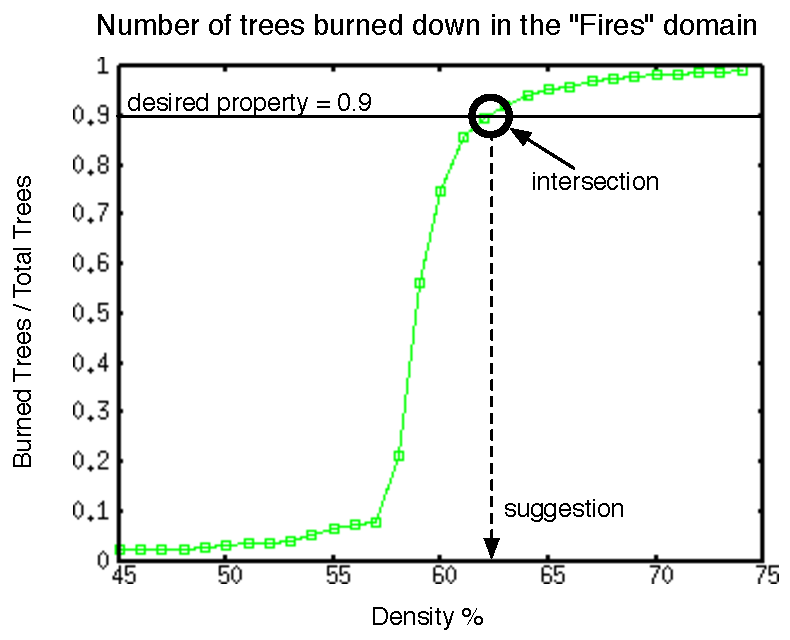
\includegraphics[scale=.66666667]{images/rii5.pdf}
\caption{The intersection between the system-level property plane 0.9 and the behavior space.}
\label{fig:rii5}
\end{figure}

When a query for a desired system-level property $p$ with value $y$ is given to RII, RII finds the intersection between the plane $p = y$ and the interpolated gradients within each hypercube.
Interpolated gradients (which are lines because the configuration space is one-dimensional) for the Fires domain are shown in Figure \ref{fig:rii3}.
This process generates a piecewise representation of the space of points that would satisfy $p=y$.
An illustration of the two planes intersecting is shown in Figure \ref{fig:rii5}.
Note that typically each hypercube's gradient does not have to be generated, like what is shown in these figures for illustrative purposes.
Only the hypercubes that intersect with the plane need to be interpolated.

% knots are the corners of a hypercube
% this is preprocessing

%example fires:


% requirements for interpolation






\subsection{Alternative: Optimization}

\subsection{Alternative: Functional Inversion}

\subsection{Special Case: Classification}


\section{Using Reverse Mappings}





\section{Evaluation Criteria}

\subsection{Time Required for Preprocessing}

\subsection{Time Required for Querying}

\subsection{Accuracy of the Reverse Mapping}


\section{Summary}




